\section{Integration Strategy}
In this section it is shown the order in which the components of the system may be integrated with each other in order to build the entire software.
As already stated, also the integration stategy follows a Bottom-Up approach and also here, the dependency relations are exploited as a guide.
For this reason, the first two components to be integrated and tested are the DatabaseAccess and the GPSService. \\
Notice that every time that it is needed to test a component which is used by other ones that have not been integrated yet, Drivers are exploited. These auxiliary “components”, the task of which is only to simulate the still missing modules, play a fundamental role because without them it would not be possible to perform Unit tests as early. \\
Another aspect to be underlined is that the Database and the GoogleMapsService, even though they are external components and so they are directly exploited without having to implement them, are however integrated as soon as possible in order to test whether their interfaces can communicate properly respectively with DatabaseAccess and with GPSService. \\
\begin{figure}[H]
\centerline{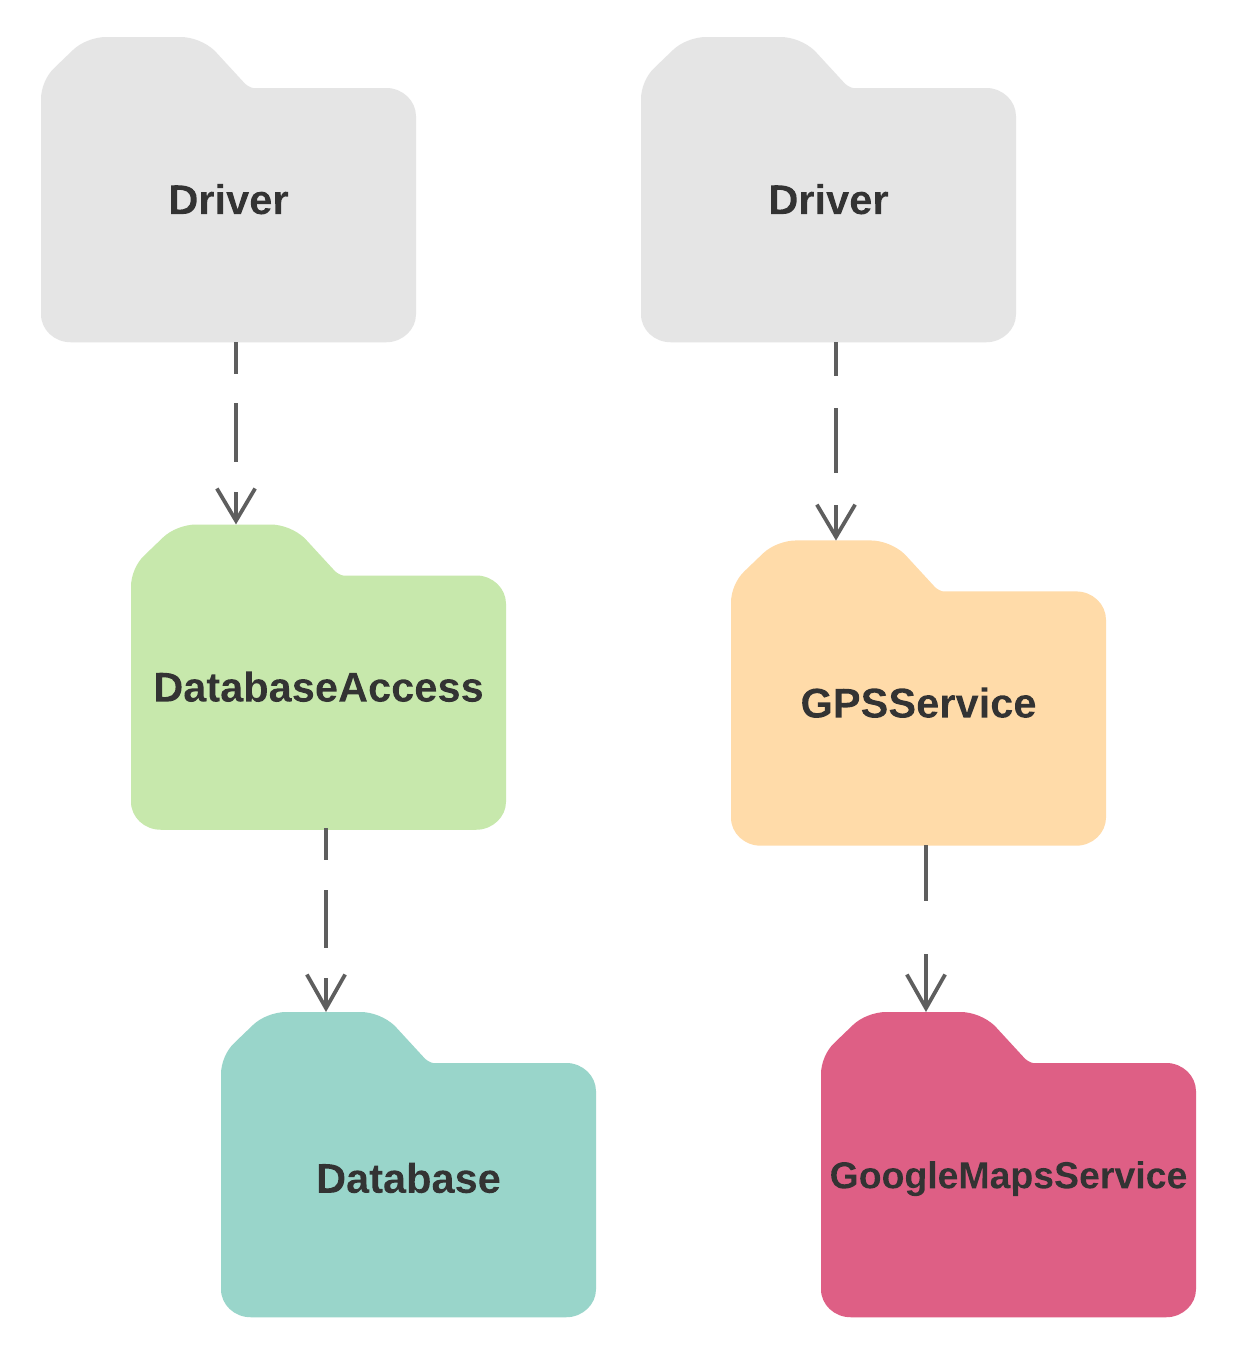
\includegraphics[scale=0.6]{./cap5/IntegrationAndTesting1}}
\end{figure}
After that, the RealTimeQueueManager can be integrated, since this component only depends on DatabaseAccess. As before, a Driver is introduced in order to simulate its functionalities and perform Unit testing. \\
\begin{figure}[H]
\centerline{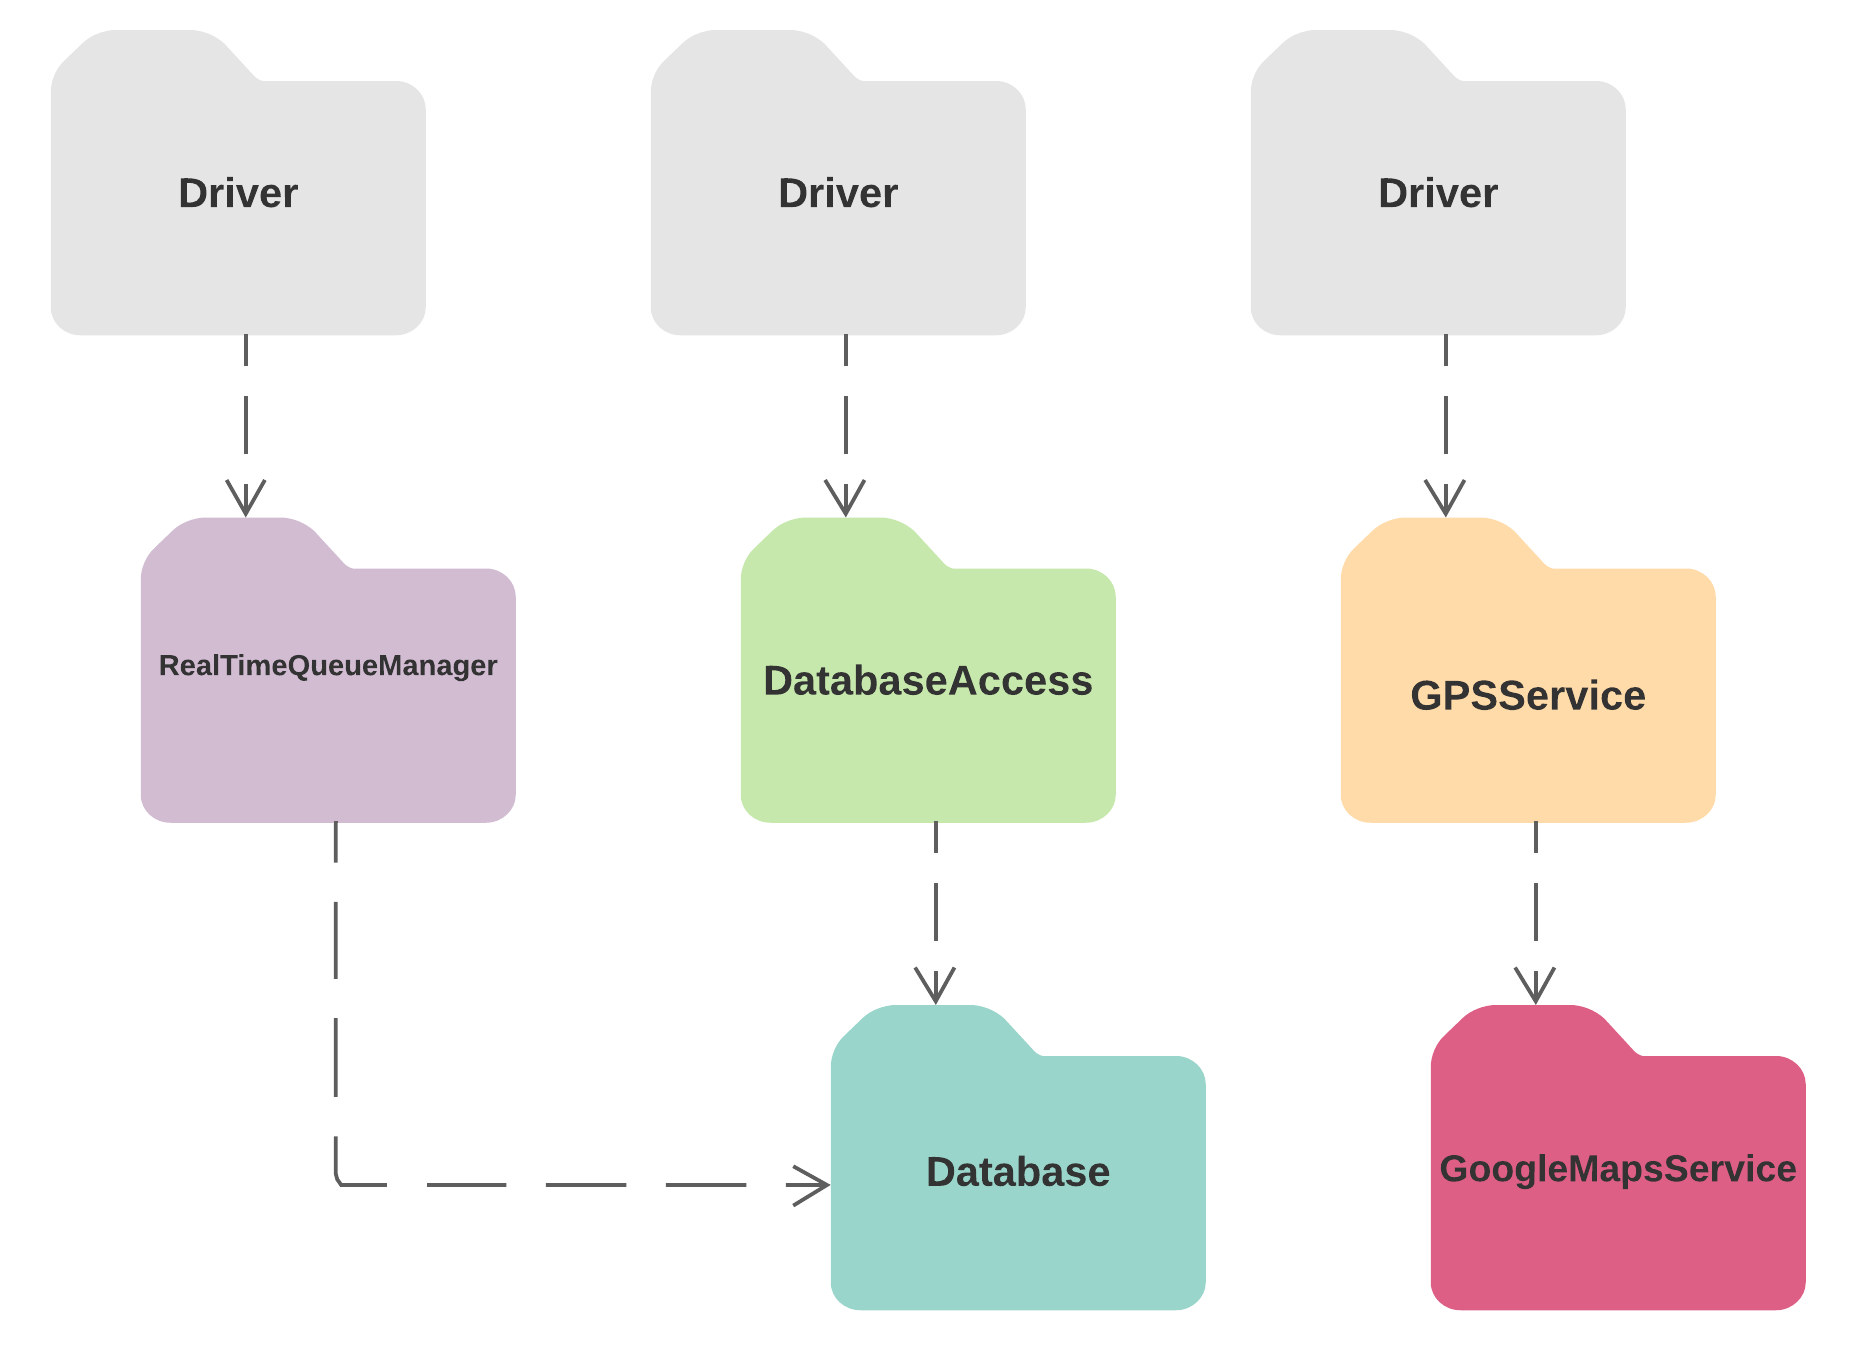
\includegraphics[scale=0.6]{./cap5/IntegrationAndTesting2}}
\end{figure}
Then, it is possible to start integrating those components that represent the Business Logic of the system. In particular, all the subcomponents of the CustomerService and StoreManagerService can be integrated. For the sake of representation, first we show only how sub-components are put together into macro-components, and then how the macro-components interact with the rest of the system. However, before doing that obviously every single sub-component is Unit tested.
So, as just stated, first the two macro-components are built. \\
\begin{figure}[H]
\centerline{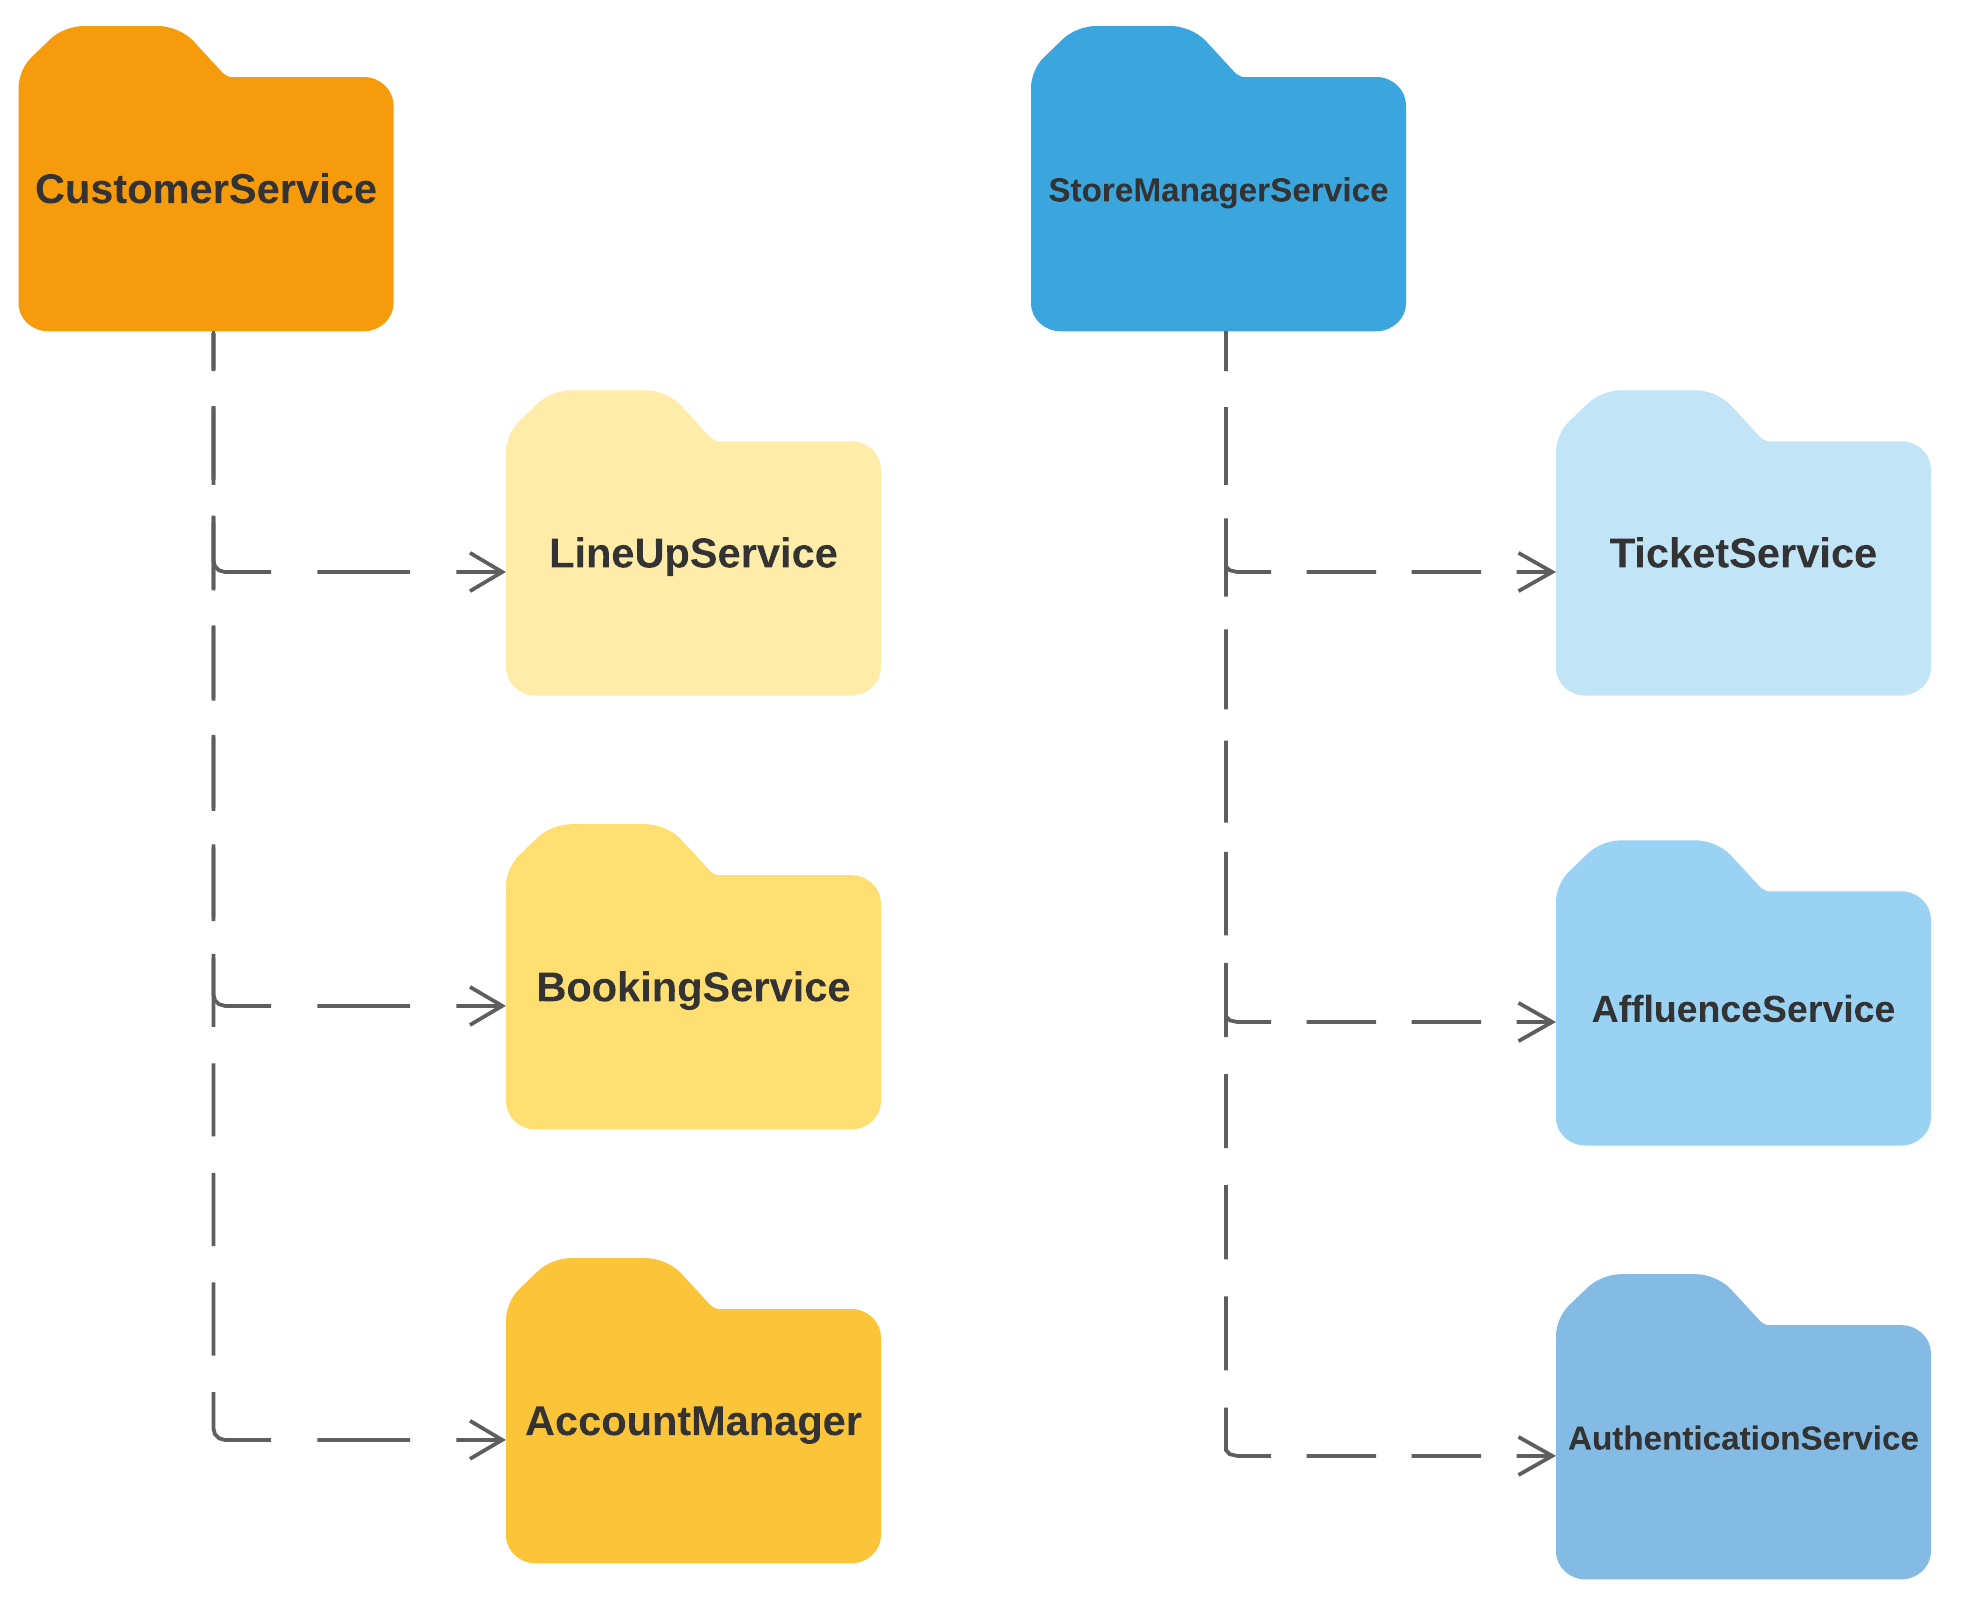
\includegraphics[scale=0.6]{./cap5/IntegrationAndTesting3}}
\end{figure}
Now that the two macro-components have been built through their sub-components, they can be integrated with the other ones. \\
\begin{figure}[H]
\centerline{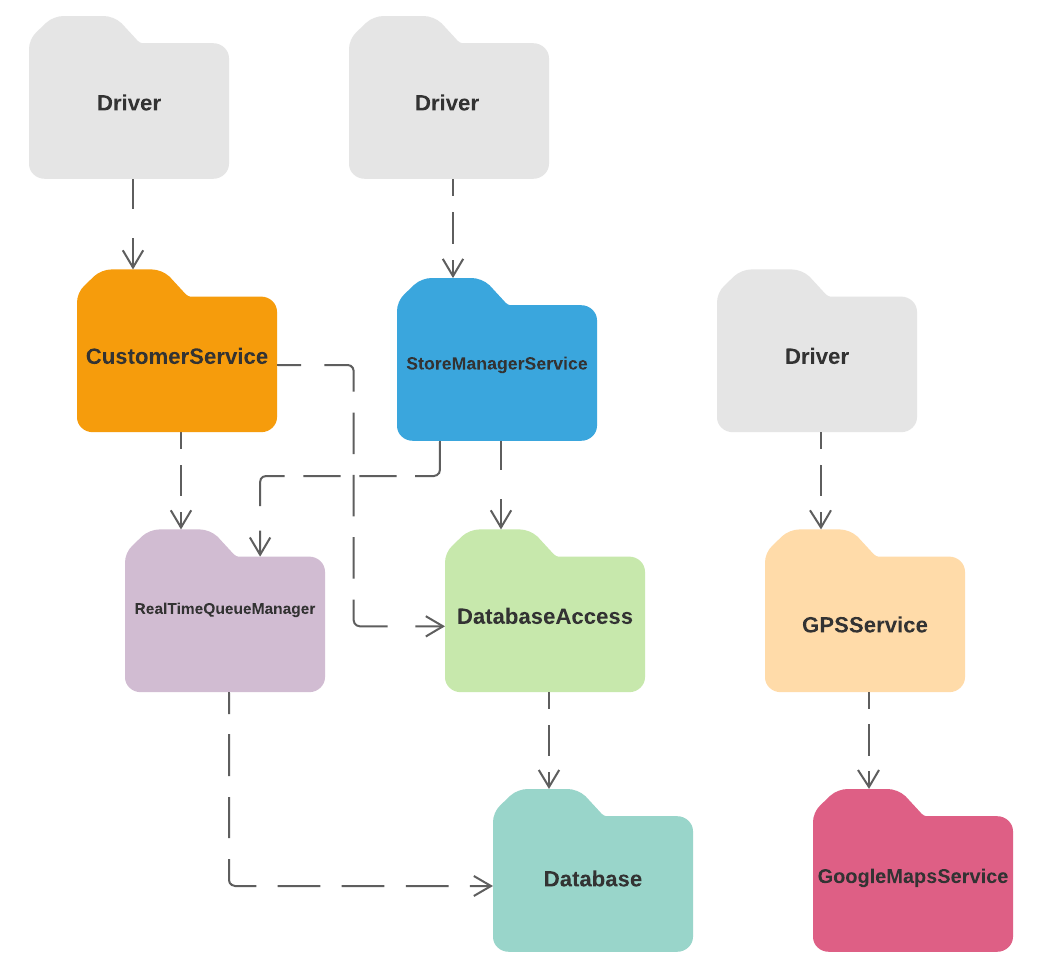
\includegraphics[scale=0.6]{./cap5/IntegrationAndTesting4}}
\end{figure}
Finally, the last two components to be integrated and tested are the WebApplication and the MobileApplication. 
\begin{figure}[H]
\centerline{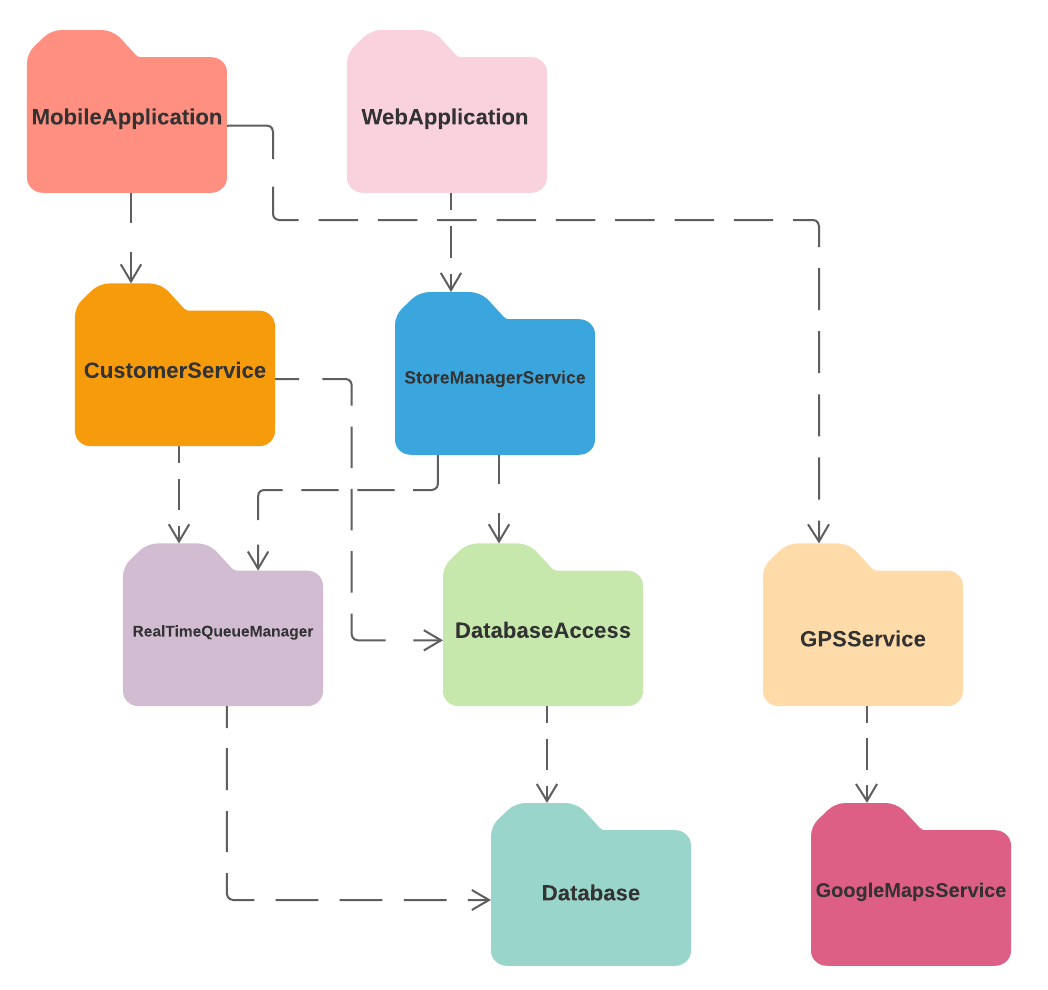
\includegraphics[scale=0.6]{./cap5/IntegrationAndTesting5}}
\end{figure}



